
%% bare_conf.tex
%% V1.4a
%% 2014/09/17
%% by Michael Shell
%% See:
%% http://www.michaelshell.org/
%% for current contact information.
%%
%% This is a skeleton file demonstrating the use of IEEEtran.cls
%% (requires IEEEtran.cls version 1.8a or later) with an IEEE
%% conference paper.
%%
%% Support sites:
%% http://www.michaelshell.org/tex/ieeetran/
%% http://www.ctan.org/tex-archive/macros/latex/contrib/IEEEtran/
%% and
%% http://www.ieee.org/

%%*************************************************************************
%% Legal Notice:
%% This code is offered as-is without any warranty either expressed or
%% implied; without even the implied warranty of MERCHANTABILITY or
%% FITNESS FOR A PARTICULAR PURPOSE! 
%% User assumes all risk.
%% In no event shall IEEE or any contributor to this code be liable for
%% any damages or losses, including, but not limited to, incidental,
%% consequential, or any other damages, resulting from the use or misuse
%% of any information contained here.
%%
%% All comments are the opinions of their respective authors and are not
%% necessarily endorsed by the IEEE.
%%
%% This work is distributed under the LaTeX Project Public License (LPPL)
%% ( http://www.latex-project.org/ ) version 1.3, and may be freely used,
%% distributed and modified. A copy of the LPPL, version 1.3, is included
%% in the base LaTeX documentation of all distributions of LaTeX released
%% 2003/12/01 or later.
%% Retain all contribution notices and credits.
%% ** Modified files should be clearly indicated as such, including  **
%% ** renaming them and changing author support contact information. **
%%
%% File list of work: IEEEtran.cls, IEEEtran_HOWTO.pdf, bare_adv.tex,
%%                    bare_conf.tex, bare_jrnl.tex, bare_conf_compsoc.tex,
%%                    bare_jrnl_compsoc.tex, bare_jrnl_transmag.tex
%%*************************************************************************


% *** Authors should verify (and, if needed, correct) their LaTeX system  ***
% *** with the testflow diagnostic prior to trusting their LaTeX platform ***
% *** with production work. IEEE's font choices and paper sizes can       ***
% *** trigger bugs that do not appear when using other class files.       ***                          ***
% The testflow support page is at:
% http://www.michaelshell.org/tex/testflow/



\documentclass[conference]{IEEEtran}
% Some Computer Society conferences also require the compsoc mode option,
% but others use the standard conference format.
%
% If IEEEtran.cls has not been installed into the LaTeX system files,
% manually specify the path to it like:
% \documentclass[conference]{../sty/IEEEtran}

\usepackage{amsmath}

% Some very useful LaTeX packages include:
% (uncomment the ones you want to load)
% ---
% PACOTES
% ---
\usepackage[english,american,brazil]{babel}		% Idioma do documento
\usepackage{color}			% Controle das cores
\usepackage[T1]{fontenc}		% Selecao de codigos de fonte.
\usepackage{graphicx}			% Inclusão de gráficos
\usepackage[utf8]{inputenc}		% Codificacao do documento (conversão automática dos acentos)
\usepackage[noadjust]{cite}
\usepackage{txfonts}			% Fontes virtuais
\usepackage{listings}
\usepackage{adjustbox}
\usepackage{tabularx}
\usepackage{multirow}
\usepackage{multicol}
\usepackage{colortbl}
\usepackage{caption}
\usepackage{microtype} 			% para melhorias de justificação
\usepackage{lipsum}
\usepackage{datetime}
\usepackage{float} %use the “float” package and then the [h] option for your figure.
\usepackage{hyperref}
\usepackage{pgf}
\usepackage{tikz}
\usetikzlibrary{arrows,shapes,automata,positioning}


\usepackage{filecontents}
% correct bad hyphenation here
\hyphenation{op-tical net-works semi-conduc-tor}

\begin{document}
%
% paper title
% Titles are generally capitalized except for words such as a, an, and, as,
% at, but, by, for, in, nor, of, on, or, the, to and up, which are usually
% not capitalized unless they are the first or last word of the title.
% Linebreaks \\ can be used within to get better formatting as desired.
% Do not put math or special symbols in the title.
%\title{Estudo e modelagem para o software de controle supervisório em veículos autônomos terrestres}
\title{Study and modeling for a supervisory control software in ground autonomous vehicles}

% author names and affiliations
% use a multiple column layout for up to three different
% affiliations
\author{
	\IEEEauthorblockN{Carlos F. de P. Perché}
	\IEEEauthorblockA{Faculdade de Engenharia Mecânica - {UNICAMP}\\
	Campinas, SP, Brasil 13083--000\\
	Email: cfpperche@gmail.com}
}

% make the title area
\maketitle

% As a general rule, do not put math, special symbols or citations
% in the abstract
\begin{abstract}

%Obter total controle das atividades em veículos autônomos terrestres continua a ser uma questão em aberto devido a crescente complexidade inerente aos demais sistemas que compõe este tipo de aplicação. Para isso, avançadas estratégias de controle supervisório devem ser desenvolvidas para que se possa fazer o uso da capacidade total destes sistemas. A principal função do controle supervisório é monitorar e coordenar as atividades dos componentes de tal forma que o comportamento geral do veículo cumpra determinados requisitos.

In this article, we present the study and modeling of an architecture for the component responsible for operational supervision over in ground autonomous vehicles and a preliminary proposal for its implementation based on formal approaches of discrete event systems and supervisory control theory. Under the proposed architecture, the supervisor control is achieved through a uniform structure of generic transitions modeled by finite state machines for the systems present in the vehicle. This structure aims to make deterministic system as a whole, facilitating the fulfillment of the requirements for the implementation of the operations performed. 

This paper proposes a solution that enables the coordination of the components which make up ground autonomous vehicles both behavioral and operational level, performing the monitoring of their software task.

%A aplicabilidade do quadro proposta é ilustrada através de um cenário simples de terreno aberto.
%The applicability of the proposed framework is illustrated by using a simple scenario of open terrain.

%Dentro deste quadro de supervisão de controle do veículo é implementado em ambos os níveis comportamentais e operacionais para a coordenação módulo, comutação comportamento do veículo, monitoramento e supervisão tarefa operação do sistema.
%Within this framework supervisory control of the vehicle is implemented at both behavioral and operational levels for module coordination, vehicle behavior switching, task monitoring and system operation supervision.


%É discutido implicação da adoção desta estrutura de transição de estado sobre a possível síntese formal de controle de supervisão.
%Implication of adopting this state-transition structure on possible formal synthesis of supervisory control is discussed.

%Esta estrutura representa um subconjunto do comportamento de cada componente que é reconhecida pelo controlador de supervisão, o qual é concebido com o objectivo de atingir um determinado comportamento do veículo.
%This structure represents a subset of the behavior of each component that is recognized by the supervisory controller, which is designed with the objective of achieving certain behavior of the vehicle.


%Sob essa arquitetura, o controle do veículo de supervisão é conseguido através uniformemente adotar uma estrutura de transição de estado "genérico" para cada componente no veículo.
%Under this architecture, supervisory control of the vehicle is achieved by uniformly adopting a "generic" state-transition structure for each component in the vehicle.


%Neste artigo, apresentamos o projeto de uma arquitetura de controle de supervisão e sua implementação preliminar de um veículo de terra capaz de operação autônoma em terreno aberto.
%In this article, we present the design of a supervisory control architecture and its preliminary implementation for a land vehicle capable of autonomous operation in open terrain.

%A estrutura é apresentada neste artigo para o controle de supervisão reforçada de tais sistemas com base em abordagens formais de sistemas de eventos discretos e teoria de controle de supervisão.
%A framework is presented in this paper for the enhanced supervisory control of such systems based on formal approaches of discrete event systems and supervisory control theory. 


%A principal função de um controlador de supervisão é monitorar e coordenar as atividades dos componentes de tal forma que o comportamento geral do veículo cumpra determinados requisitos.
%The main function of a supervisory controller is to monitor and coordinate the activities of the components such that overall behavior of the vehicle meets certain requirements.


%Resolver este problema exige não apenas componentes sofisticados para a actuação, a detecção e comunicação, mas também estratégias de controle de supervisão avançados que podem fazer uso da capacidade total dos componentes.
%Solving this problem requires not only sophisticated components for actuation, sensing, and communication, but also advanced supervisory control strategies that can make use of the full capability of the components. 


%Alcançar operação autônoma por um veículo não tripulado em terreno aberto continua a ser um problema desafiador no desenvolvimento de veículos terrestres.
%O controle de supervisão de veículos terrestres não tripulados, devido à sua crescente complexidade inerente tornou-se um componente muito importante.

%Achieving autonomous operation by an unmanned vehicle in open terrain remains a challenging problem in the development of land vehicles. 
%The supervisory control of unmanned ground vehicles due to their inherent growing complexity has become a very important component.
\end{abstract}

\begin{IEEEkeywords}
unmaned land vehicle, supervisory control, finite state machine, critical real-time system, discreve event system.
\end{IEEEkeywords}


\IEEEpeerreviewmaketitle
% -------------------- NEW SECTION -------------------- 
% -------------------- NEW SECTION -------------------- 
% -------------------- NEW SECTION -------------------- 
\section{Introduction}\label{sec:introduction}
Autonomous land vehicles need to be equipped with a variety of components for processing data, communication, actuation, sensing, etc. The complexity of these components has grown and increasingly they perform their duties independently. Once the components are properly integrated and coordinated, they can make autonomous navigation guiding the vehicle with minimal human intervention \cite{autonomous_Hebert:1997:IUG:523961}.

Achieve autonomous behavior in a land vehicle still remains a challenging issue, mainly due to the complexity of the operating environment presents. The Earth's surface as well as climatic reasons, has a large variety of features that make up the manual navigation difficult. These conditions significantly interfere with the performance of land vehicles \cite{supervisory_Donmez:2010:MSE:2377576.2377580}.

The solution for such problems require beyond the use of sophisticated components for processing, communication, actuation and sensing, but also a good strategy for supervisory control can enable the components can use the best of their ability, without significant degradation in performance of the system \cite{supervisory_Cummings_1a}. The main function of a supervisory system is the monitoring and coordination of activities running on components so that the vehicle meets the certain goals, which may range from moving from one place to another as fast as possible, or simply follow another vehicle in front to a safe distance.

Also, we must take into account that this type of application is characterized as a critical real-time system \cite{rtos_safety_mission_4062424}, %
where alternatives to ensure that certain tasks are fulfilled in a specified time period, otherwise severe failures will occur, making the project unfeasible \cite{rtos_nasa_monitors}. %\cite{rtos_choosing_barr2003choosing} \cite{rtos_analysis_336046}.

This work presents the proposal of the supervisory control architecture for the Intelligent Vehicle of the Autonomous Mobility Lab (VILMA) \cite{lma_vilma_website} and its development process, aimed at obtaining autonomous operations in land environments, taking into account the requirements for critical real-time systems. Under the proposed architecture, we adopted a uniform interface that should be incorporated into systems that make up the vehicle as well as a platform that enables the development of the project. The interface adopted represents a behavioral set, wherein each component present in the vehicle architecture can have their tasks managed by the supervisor, enabling the operations performed by the vehicle have deterministic character.

The rest of the paper is organized as follows. Section \ref{sec:architec_riquirements} describes the concepts and methodologies used to the architecture of supervision and lists the goals and desired requirements. Section \ref{sec:proposed_architec} describes the general behavior of VILMA autonomous vehicle, shows the modules and components present in vehicle architecture, describes the state transitions structure for the tasks to be performed on a component, where the supervisory control strategies act according to expected behavior and discusses a possible methodology for a formal synthesis of control for the proposed architecture. Section \ref{sec:architec_components} presents the software elements used in the architecture development platform.
Section \ref{sec:implementation} discusses a preliminary description to implement the supervisory control architecture. Section \ref{sec:conclusion} concludes this paper.

% -------------------- NEW SECTION -------------------- 
% -------------------- NEW SECTION -------------------- 
% -------------------- NEW SECTION -------------------- 
%\section{Architecture Concepts}\label{sec:architec_concepts}
\section{Architecture Requirements}\label{sec:architec_riquirements}

%Um veículo autônomo terrestre (VAT) é composto por diversos sistemas que possuem funções específicas, como percepção do ambiente local, controle da navegação, localização global, etc., todos operando em paralelo. 

According to \cite{autonomous_siegwart2011introduction}, autonomous systems must have three basic operations: which are perception, location, and environment mapping; path planning and movements control. Typically a VAT has three operating modes: manual, autonomous and collaborative mode, the latter consists of ADAS (Advanced Driver Asssited Systems).

%Tipicamente um VAT possui o modo de operação manual, forma convencional com que os veículos são operados, e modo autônomo, que possui um completo controle computacional que determina sua "inteligência".

The advancement of research involving VAT has resulted in an increased level of complexity and amount of data in their specific sensors and systems, creating the need to distribute information processing in various "embedded computers" that communicate synchronously. Thus, a appropriate supervision of vehicle modules is essential to a modular design with deterministic characteristics. This management should perform the control according to the needs of each task activities and ensure the vehicle behavior based on rules that prioritize safe operations.

%Além disso, o desenvolvimento de um VAT necessita ser adaptável para todos os requisitos funcionais nos diversos cenários de operação em que o veículo possa realizar suas tarefas. Neste contexto, o sistema controle supervisório precisa verificar a integridade dos demais módulos que realizam, por exemplo, a leitura dos sensores, o controle de velocidade ou o sistema de posicionamento. Ou seja, verificar constantemente a presença e o comportamento destes sistemas.

Formal techniques such as finite state machines (FSM) to model the behavior of deterministic systems and get your supervisory control has been used in various areas including network communication, traffic control systems, assembly lines, and so on \cite{event_comparative_study} \cite{event_des_line_945770}. This same technique has been presented by researchers in related work, such as robotic applications and autonomous vehicle systems. \cite{event_supervisory_soccer_994642} uses a set of FSMs to describe the robot collaborative behavior to football matches. \cite{event_hybrid_automata_827799} models the operations of an autonomous robot using a hybrid system of automata, on which the changes of their behavior is modeled by FSMs containing discrete states which correspond to distinct behaviors through a continuous model. \cite{event_modular_navigation} presents an application where their behavior is based on modeling state machines for a modular navigation system in a vehicle that operates under tunnels.

The described works aims to model the behavior between the switching of activities to accomplish its tasks, making the vehicle or the robot's behavior strictly deterministic. However, the issue about dynamic reconfiguration of the systems to that they can work in changing environments is not addressed. In addition, these studies do not take into account the problem of coordination among the components that make up the architecture of their robotic systems. While there is great progress in addressing research methods of perception, vision, positioning, navigation, trajectory planning, control, etc., research and applications dealing supervision platforms for autonomous systems are not at the same level. \cite{event_supervisory_land_1157827} presents an architecture and preliminary implementation for the supervisory system of VAT called Ulysses.

%\begin{figure}[h]
%	\centering
%	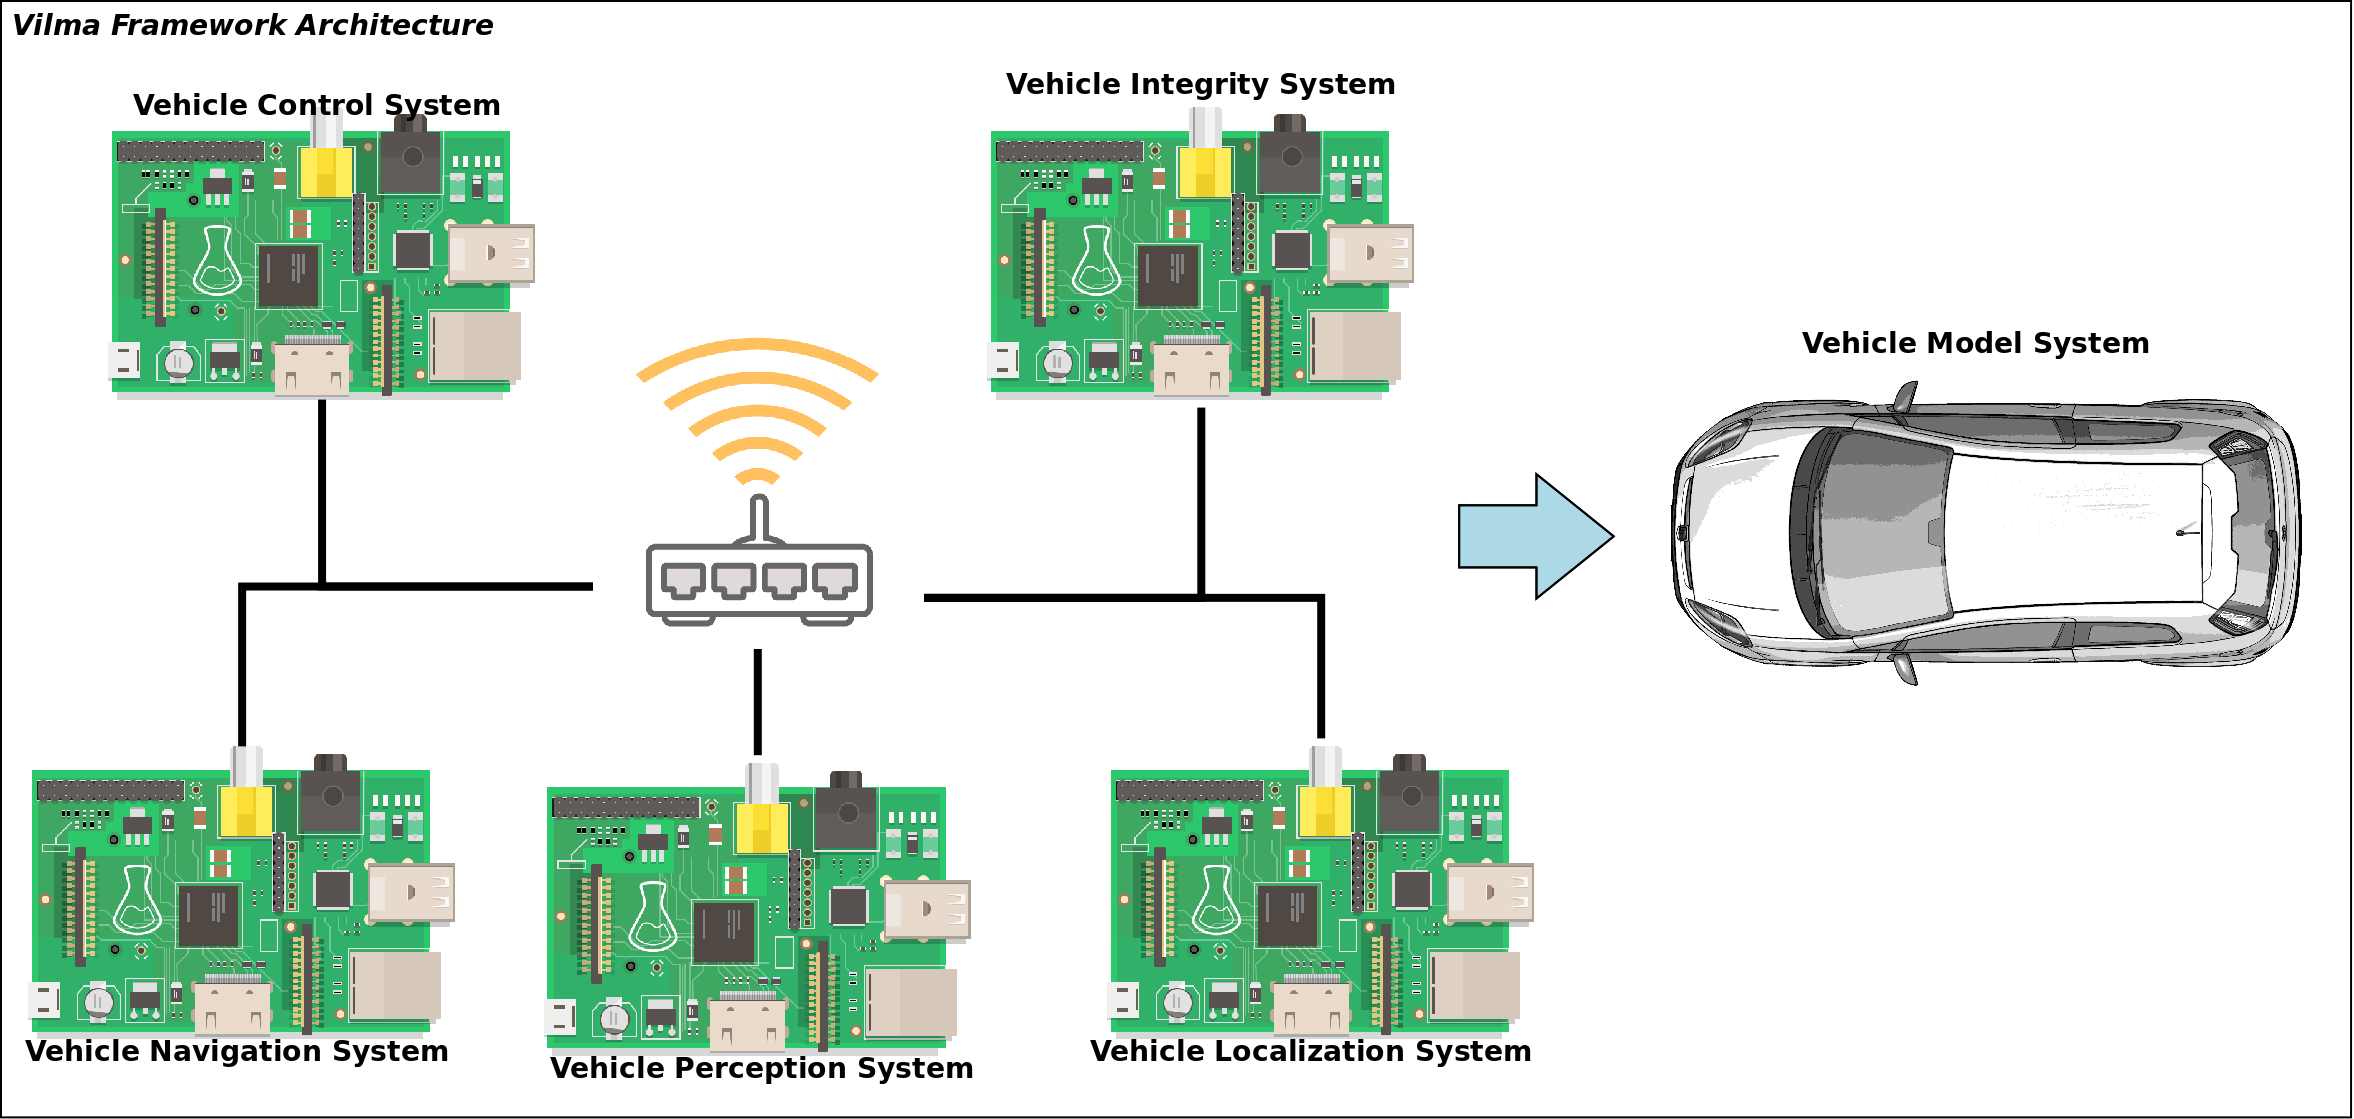
\includegraphics[width=200px,keepaspectratio]{imagens/VILMA_SYSTEM_ARCHITECTURE2}
%	\caption{Processamento descentralizado.}
%	\label{fig:VILMA_SYSTEM_ARCHITECTURE}
%\end{figure}

Having as main objective of this study, the development of a supervisory system called "Vehicle Integrity System" (VIS), part of the VILMA project, responsible for checking and control vehicle operating modes, monitor the states of the other modules, supervise and coordinate systems in different operating modes, propose decision-making in case of failure of any components, perform control and message log for easier system maintenance and debugging during the project development phase. To meet the goal of the work, the proposed architecture must ensure the following requirements:


Tendo como principal objetivo deste estudo, o desenvolvimento de um sistema denominado "Vehicle Integrity System" (VIS), parte do projeto VILMA, responsável por verificar e controlar os modos de operação do veículo, monitorar os estados dos outros módulos, supervisionar e coordenar os sistemas nos diferentes modos de operação, propor a tomada de decisões em caso de falhas dos componentes presentes na arquitetura do veículo, realizar o controle e registro de mensagens facilitando a manutenção e depuração do sistema durante a fase de desenvolvimento do projeto. Onde, para de atender o objetivo do trabalho, a arquitetura proposta deve garantir os seguintes requisitos:

\begin{itemize}
	\item propose an architecture with deterministic characteristics for the development of critical real-time systems;
	\item standardize the communication interface between the systems present in the vehicle architecture;
	%\item fornecer uma interface que possibilite a integração de outros trabalhos ao sistema supervisório de forma ágil e baixa complexidade;
	\item provide a supervisory system which monitors the current state of other vehicle components;
	\item the supervisory system should collect information about the other components, which should be reported to the user interface of the vehicle;
	%\item o supervisor deve decidir se um componente está trabalhando de forma esperada ou não, e tomar decisões para solucionar problemas;
	\item in addition to the behavioral control and operational management, the supervisory system must monitor the health of the other components that implement the interface provided by VIS;

%	\item to ensure a set of characteristics that the architecture of all the built robots will provide. For example, the real-time communication bandwidth guarantee for a n number of dispositives plugged into the robot;
	
	%\item to manage the interface between the real-time requirements of the manipulation tasks of the robot and the non-realtime computational intelligent process of the decision algorithms;
	
	%\item to standardize the communication interfaces among the robot dispositives and to standardize the communication interfaces among the main parts of the robot;
	
	%\item to develop an architecture capable of integrating and validating new technologies, such as different kinds of actuators and sensors;
\end{itemize}


% -------------------- NEW SECTION -------------------- 
% -------------------- NEW SECTION -------------------- 
% -------------------- NEW SECTION -------------------- 

\section{Proposed Architecture}\label{sec:proposed_architec}

This paper proposes a system for supervisory control using the conventional concept of modeling FSM taking into account the problem of dynamic reconfiguration for the VILMA vehicle as a potential development platform to other research developed in the LMA. The formal concepts for modeling FSM and DES to the supervisory system are adopted to perform the cordination of the other modules, exchange vehicle operating mode, monitoring the integrity of systems and management of the operating states of the modules.

The supervisory control is able to manage only what the other systems are reporting to him, to do this, there needs to have a common interface between modules in the vehicle, which in case of a malfunction or the occurrence of unexpected behavior the supervisory system can perform the coordinating of the other systems to react to a potential situation. The proposed platform may be considered as a copilot type from the VAT that tells the vehicle as their activities must be organized, which configuration to use at a particular time, while displaying failures detected on a specific system, etc.

%
% operational_modes
\subsection{Operational Modes}\label{subsec:operational_modes}

The Autonomous Mobility Laboratory (LMA) develops research in order for the VILMA project can perform tasks for the manual and autonomous operation modes. In the manual mode, the vehicle is driven by a human operator in a conventional manner. In the autonomous mode, the vehicle is driven by a computer control system that receives data from your sensors, processes the information collected and acts directly on its mechanical actuators. Once in autonomous mode, the vehicle is expected to perform tasks without direct human intervention. The realization of the autonomous operations are characterized by a subset of operational modes, named as: \textit{Open Terrain}, \textit{Road Following}, \textit{Vehicle Following} and \textit{Teleoperation}.

\begin{itemize}
	\item \textit{Open Terrain}, the vehicle operates in open environments, ie any type of terrain that has valleys, depressions, deserts, etc;
	\item \textit{Road Following}, vehicle moves along a road being guided by the features present in this road, for example, boards, traffic lights, etc.;
	\item \textit{Vehicle Following}, the vehicle must simply follow another car in front;
	\item \textit{Teleoperation}, the vehicle must perform tasks remotely controlled;
\end{itemize}

%A troca entre o modo de operação manual para o modo autônomo é feita diretamente pelo operador dentro do veículo. Uma vez que o automóvel encontra-se em modo autônomo, o condutor pode realizar a troca para o modo manual quando necessário ou assim que desejar.

%Durante o desenvolvimento do projeto o veículo deve executar suas tarefas operando em modo de depuração, nesta fase é possível operar em modo autônomo sendo permitida a realização de testes dos componentes e módulos que sendo desenvolvidos, porém o controle manual deve estar sempre disponível ao operador, tendo prioridade superior a qualquer tarefa autônoma sendo executada. A depuração também deve contar com o sistema de registro e visualização das mensagens e o estado sobre a situação atual de cada módulo em execução. A Figura \ref{fig:VILMA_OPERATIONAL_MODE} ilustra os modos de operação e as possíveis trocas entre os modos.

%\begin{figure}[h]
%	\centering
%	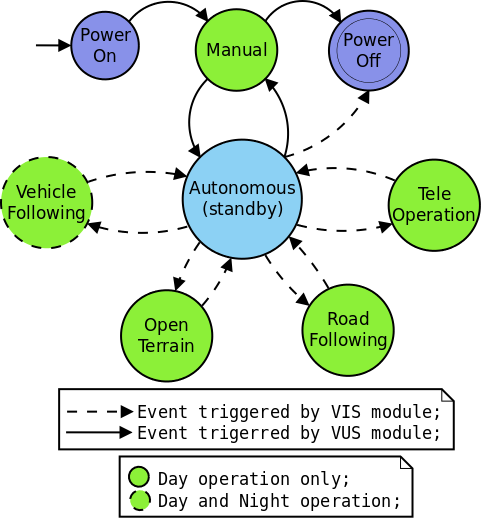
\includegraphics[width=200px,keepaspectratio]{imagens/VILMA_OPERATIONAL_MODE}
%	\caption{Modos de operação do projeto VILMA.}
%	\label{fig:VILMA_OPERATIONAL_MODE}
%\end{figure}

%O mecanismo de comutação entre modos operacionais é composto por um conjunto de funções que todos os módulos da arquitetura do veículo devem obedecer para que as tarefas sejam executadas sem comprometimento das atividades. Isso permite ao veículo ter o comportamento esperado, por exemplo, quando cada módulo estiver no estado \textit{Working}, então, estes módulos estarão prontos para executar funções específicas para cada um de seus sistemas. No entanto, pode haver o caso em que funções específicas a determinados modos de operação precisem ser combinadas para possibilitar que tarefas complexas sejam cumpridas de forma eficiente. Por exemplo, o módulo de navegação possui funções que realizam tarefas específicas nos modos de operação \textit{open errain} e \textit{road following}. A combinação dessas duas funções vai gerar uma nova funcionalidade, resultando em um novo comportamento durante seu deslocamento. Ainda tendo como exemplo o sistema de navegação, as informações captadas pelos sensores do módulo de localização e percepção (GPS, IMU, Bussola, Câmera, Laser Escâner, etc.) é que determinam quando deve ser feita a alteração entre os modos operacionais. 

%Para exemplificar, considere a seguinte situação, suponha que o veículo esteja operando em modo \textit{open terrain}, e em algum momento o veículo recebe uma requisição do sistema de usuário para alterar seu destino. Neste momento, o sistema de usuário deve informar ao supervisório que houve uma requisição para alterar o destino da missão, consequentemente o supervisório direciona a informação para que o sistema de navegação instrua os sistemas de localização e posicionamento que continuem operando em modo \textit{open terrain}, caso a nova rota traçada possua uma estrada (detectada pelo tratamento das informações obtidas nos sensores), então os sistemas são informados que há uma estrada que leva ao destino e então devem alterar modo de operação adequado à aquela situação, no caso, \textit{road following}.

%Podemos dizer que o veículo possui um sistema "inteligente" capaz de fornecer um conjunto abrangente de funções através da conjunção de funcionalidades, onde esta inteligência pode ser modelada por maquinas de estados para possibilitar o comportamento esperado pelo sistema supervisório, como no exemplo apresentado pela Figura \ref{fig:VILMA_OPERATIONAL_MODE_BEHAVIOR}.

%\begin{figure}[h]
%	\centering
%	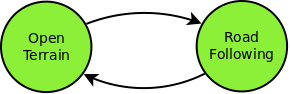
\includegraphics[width=120px,keepaspectratio]{imagens/VILMA_OPERATIONAL_MODE_BEHAVIOR}
%	\caption{Comportamento de comutaçao FSM dos modos de operaçao.}
%	\label{fig:VILMA_OPERATIONAL_MODE_BEHAVIOR}
%\end{figure}

%
% modules_components
\subsection{Modules and Components}\label{subsec:modules_components}

The development of systems with a modular architecture aims to improve quality of the software, decrease the time required to integrate new features and speed up the delivery of the work. For this reason, VILMA vehicle is basically composed of seven systems, also called modules. Each system and consists of components that perform specific tasks. The modules and some of the main components present in vehicle architecture can be seen in the Figure \ref{fig:VILMA_MODULES_COMPONENTS}.

\begin{figure}[h]
	\centering
	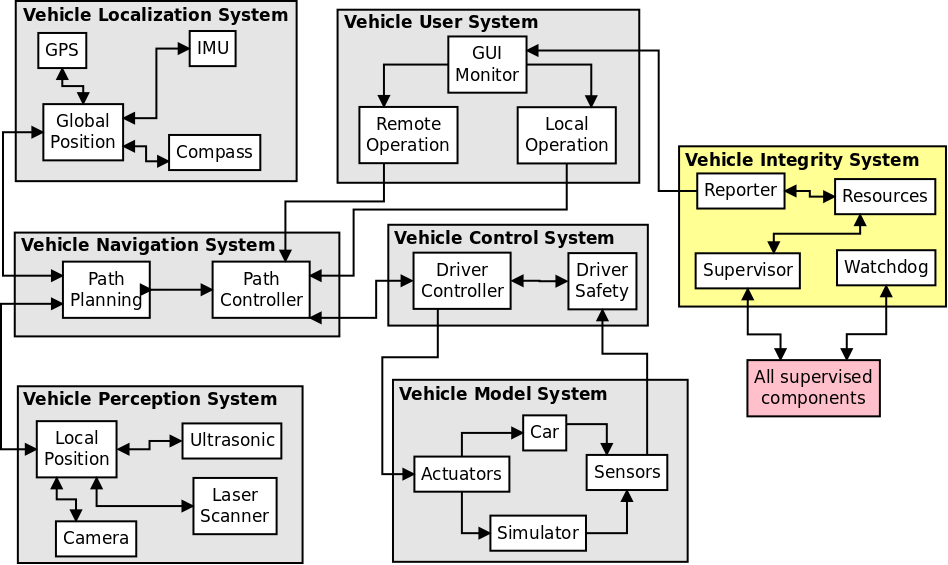
\includegraphics[width=270px,keepaspectratio]{imagens/VILMA_MODULES_COMPONENTS}
	\caption{VILMA modules and components.}
	\label{fig:VILMA_MODULES_COMPONENTS}
\end{figure}

The list below introduces an overview of the modules and its main functions to the VILMA project.

\begin{itemize}
	\item \textit{Vehicle Model System} (VMS): It is the system that represents the vehicle, both real and simulated, it implements the interface between the actuators and the low-level sensors, which the actuators receive commands from VCS system to perform any tasks and feedback signals generated by the sensors are sent to own VCS;
	
	\item \textit{Vehicle Control System} (VCS): Module responsible for to control the actuation of the vehicle and ensure the safety of those involved in the operating environment. Its main function is to provide commands to the speed control, acceleration and vehicle direction. The VCS generates low-level signals that trigger the electromechanical system, telling the desired speed, the acceleration needed and the angle of direction. Moreover the VCS system, has a cyclical feedback communication with the VNS system to ensure that the speed and direction commands are both running correctly, taking into account environmental factors such as wheel slippage and others.
	
	\item \textit{Vehicle User System} (VUS): The VUS module enables the interaction of the driver to the car, both in local mode and in remote mode, enabled by using cameras mounted on the vehicle to simulate the driver's view. The operator controls the movement of the car through a remote control. Furthermore the system should provide a graphical interface enabling the driver to know the state of the vehicle in the real time as well as provide alerts and diagnostics for debugging during development stage.
	
	\item \textit{Vehicle Perception System} (VPS): The VPS system uses several instruments such as laser scanners, cameras, ultrasonic sensors, etc. to construct digital maps of the environment around the vehicle, it provides the local position of the vehicle. The generated map is sent to the VNS system, which performs the planning of the trajectory and the generation of the movement commands to the VCS system.

	\item \textit{Vehicle Localization System} (VLS): Just like the VPS system, the VLS module uses several instruments such as GPS, IMU, electronic compasses and other sensors that make possible the generation of digital maps of their location on a global scale. It also gives the map information generated for the VNS system to be able perform of path planning and generation of the movement commands to the VCS system.
		
	\item \textit{Vehicle Navigation System} (VNS): It is responsible for generating commands to the vehicle navigation in order to perform the task specified by the operator. Furthermore it must to be able to carry out the planning of the path to the desired location, calculate the speed and its heading, generating the necessary information in order to the VCS system to perform the tasks safely.

	\item \textit{Vehicle Integrity System} (VIS): The VIS module is responsible to ensure the integrity of the system that operates the vehicle while it is running. Its main function is to monitor and coordinate the activities of the modules to achieve the expected behavior of the vehicle. The VIS must also perform routing of data between the other modules, registers and publishes the information which contains the status of the systems. In short, the VIS acts as a digital copilot. Further description of the supervisory system will be presented in this paper.
\end{itemize}
%
% states_transitions
\subsection{States and Transitions for Supervisory Control}\label{subsec:states_transitions}

In order to have the proper coordination between the activities performed by the present systems in vehicle architecture, it is necessary that the components have a uniform behavior in relation to the VIS system. Thus, each component needs to implement a common interface, modeled by a set of states and transitions that are recognized by the supervisory system, enabling the management of their activities being performed, perform routing of messages required for debugging and the data storage, etc. The coordination of the modules is responsible for determining the sequence of activities and the conditions that a system must have so that it can perform its specialties.

Under the perspective of supervisory control, the states present in the common interface of the systems are: PowerOn, Standby, Ready, Working, InternalError, Emergency, Shutdown and PowerOff. Each component must contain these states. For a certain component, the meaning of the states and the general behavior of the vehicle can be summarized as follows.

\begin{itemize}

	\item \textit{PowerOn} The driver starts the vehicle, at this moment the engine is started but the car remains parked awaiting the instructions of the driver. 
	
	\item \textit{Standby} The component comes to be started and the vehicle remains stationary. In this state, the system is not linked to an autonomous operation mode, it remains awaiting the instructions from the supervisory system about the operating mode that it will work or the instruction to return to the manual mode;
		
	\item \textit{Ready}, In this state the component is linked to an autonomous operation mode but not yet operated in this mode. The reason for the separation between Standby and Ready states is due to the fact that the article focuses on the general behavior of the vehicle, clearly denoting the temporal separation of the states which the vehicle can return to manual operation and the state which it is ready to operate in standalone mode. The temporal separation of the states is required for the synchronization of activities on the components before they enters in the state Working.
	
	\item \textit{Working}, In this state the component is operating in a autonomous mode and the vehicle is moving. Now, the algorithm that performs specific functions of the component begins to run to produce its expected behavior.

	\item \textit{InternalError} e \textit{Emergency} The component performs tasks relevant to handling exceptions raised by your specific algorithm or handling of emergency that might compromise the overall operation of the vehicle.
		
	\item \textit{Shutdown}, The component executes a predefined set of routines preparing the vehicle to be turned off, bringing the system to the state PowerOff;
	
	\item \textit{PowerOff}, The system is turned off and no electric signal is supplied to the component.
\end{itemize}

Transitions between states are a set of activities that lead the components from one state to another. In order to a transition occurs it must be triggered by an event. Once invoked, the activities associated with the transition must be performed successfully so that the component get into a new state. The diagram of the common states and transitions to the supervisory system can be seen in Figure \ref{fig:VILMA_STATE_MACHINE2}. Specifications that represent constraints of the activities for each module may also be modeled by automatas to produce a composite  specification model. With the obtained model, based on the theory of control for discrete events (DES) we can get a formal model for supervisory control, as discussed in \cite{event_systems}.

The resultant specifications, described by an FSM form a chain containing all activities and sequences of allowed transitions to ensure that all specifications are fulfilled, i.e., when any of the modules need to perform a transition between states of the FSM that describes its behavior. For example, to enter the Working state or leave the Working state and go to the Standby state or when a module is performing the treatment of some exception in InternalError, all transitions of related states must check their restrictions and obtain permission from the the supervisor module before the transition occurs.

\begin{figure}[h]
	\centering
	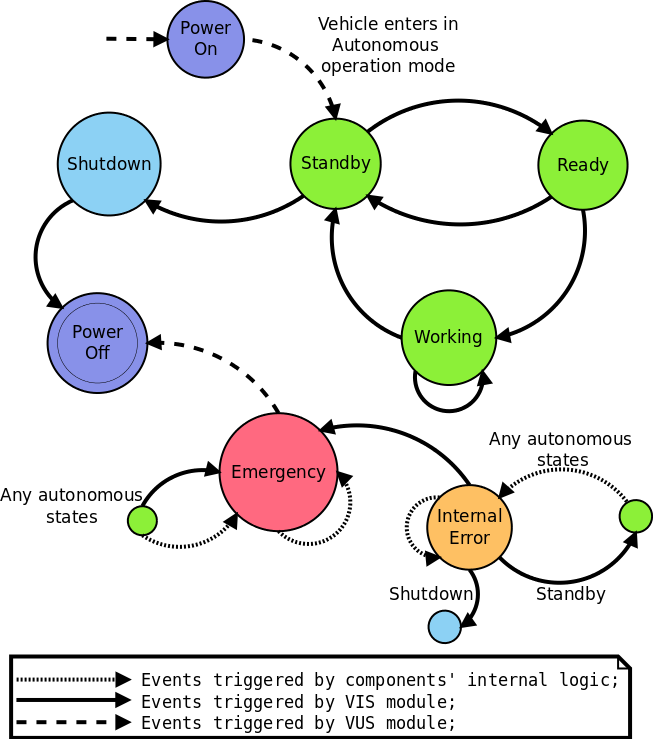
\includegraphics[width=250px,keepaspectratio]{imagens/VILMA_STATE_MACHINE2}
	\caption{States and transitions of components.}
	\label{fig:VILMA_STATE_MACHINE2}
\end{figure}

Although each component contains the set of states and transitions required, the question of the activities involved in the states and transitions is transparent to the VIS. In other words, the VIS not internally knows the complexity of the tasks performed within the states or during the transitions from one component and there is no restriction that it only has these states and transitions. The activities involved in the transitions of each component may differ from those present in other components.
%
% formal_synthesis
\subsection{Approach of DES on Formal Synthesis }\label{subsec:formal_synthesis}

After modeling pattern that determines the behavior of the modules in terms of states and transitions, it is possible to synthesize logic of VIS by formal techniques, for example, the supervisory control theory to discrete event systems \cite{event_systems}. The application of this technique requires that the states and transitions of the modules are expressed by sets of automata (called models), while the desired behavior of the vehicle is expressed by other sets of automata (called specifications). For example, the behavior of a module, according the specifications of the VIS as illustrated in Figure \ref{fig:VILMA_STATE_MACHINE2}, can be represented by an automata $G = (Q,\Sigma,\delta,q_{0},Q_{m},q_{m-1})$, where, $Q$ is a set of states, e.g., $Q =$ \{\textit{PowerOn, PowerOff, Standby, Ready, Working, InternalError, Emergency, Shutdown}\}, $\Sigma$ is a set of transitions, e.g., $\Sigma =$ \{\textit{1,2,3,4,5,6,7,A,B,C,D,E,F,G,H,I,J,K,L,$\alpha$,$\beta$,...}\}, $\delta$ is a transition function that specifies the new state after a transition from a given state, as presented in Table \ref{tab:func_transicao}, $q_{0}$ is the initial state of the component, $q_{m-1}$ is the final state of the component and $Q_{m}$ is the set of states that indicate the completion of certain desired sequence of tasks.

% Please add the following required packages to your document preamble:
% \usepackage{multirow}
\begin{table}[h]
	\centering
	\adjustbox{max height=\dimexpr\textheight-5.5cm\relax, max width=\textwidth}{
		\renewcommand{\arraystretch}{1.1}
		\begin{tabular}{|c|c|c|}
			\hline
			\multicolumn{3}{|c|}{$\delta(old state, transition) = new state$} \\ \hline
			Old state & transition & new state \\ \hline
			power-on & A & standby \\ \hline
			\multirow{4}{*}{standby} & B & ready \\ \cline{2-3} 
			& C & shutdown \\ \cline{2-3} 
			& D & internal error \\ \cline{2-3} 
			& E & emergency \\ \hline
			\multirow{4}{*}{ready} & F & working \\ \cline{2-3} 
			& G & standby \\ \cline{2-3} 
			& H & internal error \\ \cline{2-3} 
			& I & emergency \\ \hline
			\multirow{4}{*}{working} & J & standby \\ \cline{2-3} 
			& K & working \\ \cline{2-3} 
			& L & internal error \\ \cline{2-3} 
			& M & emergency \\ \hline
			\multirow{3}{*}{internal error} & N & standby \\ \cline{2-3} 
			& O & shutdown \\ \cline{2-3} 
			& P & internal error \\ \hline
			\multirow{2}{*}{emergency} & Q & power-off \\ \cline{2-3} 
			& R & emergency \\ \hline 
			shutdown & T & power-off \\ \hline
		\end{tabular}
		\renewcommand{\arraystretch}{1}
	}
	\caption{Example of the transition function $\delta$ of the model based on the Figure \ref{fig:VILMA_STATE_MACHINE2}.}
	\label{tab:func_transicao}
\end{table}

Since each module of the system is modeled by an automaton $G_{i}$, a composite model of the overall behavior of the vehicle can be build using the procedure called "synchronous product", represented by the symbol $\lVert$ \cite{event_systems_ebook}. The result of the synchronous product over all $G_{i}$ is a new automaton that represents the "free" behavior (uncontrolled) of simultaneous activities of the components, i.e., $G = G_{1} \lVert G_{2} \lVert G_{3} \lVert ... \lVert G_{n}$.  

Then the desired deterministic behavior of the vehicle may be imposed on the behavior "free" to obtain strategies for supervisory control expected by the VIS system. Formally, such behavior is also expressed in automata, called specifications automata. By imposing the specifications of the model composite of all vehicle components, a sequential set of transitions may be obtained to be run by the VIS, ensuring that the vehicle behavior control meets the specifications.

By using this approach, it is possible to synthesize the supervisory control strategies that allow the vehicle to deal with different situations. For instance, suppose that, due to timing synchronization constraints, the VCS can only enter the Working state  after VNS is in Working state. This can be considered as a requirement to comprise the desired behavior for the initialization of a task. This requirement can be expressed as a specification $S_{i}$, as shown in Figure \ref{fig:VILMA_TRANSITION_EXAMPLE}, which the cyclic loops represent other possible transitions that can occur in the system.

\begin{figure}[h]
	\centering
	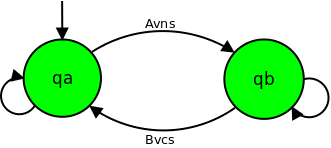
\includegraphics[width=120px,keepaspectratio]{imagens/VILMA_TRANSITION_EXAMPLE}
	\caption{Specification example, $A_{vns}$: Transition from \textit{Ready} state to \textit{Working} in the \textit{Vehicle Navigation System} module, $B_{vcs}$: Transition from \textit{Ready} state to \textit{Working} in the \textit{Vehicle Control System} module.}
	\label{fig:VILMA_TRANSITION_EXAMPLE}
\end{figure}

The supervisory control that guarantees the behavior of the modules as a whole, and meets the specification imposed by $S_{i}$ can be obtained, among other ways, by the algorithm \textit{SUPCON} \cite{supcom_wonham1987supremal}. Their function is to generate sequences of events as another automaton $V$, i.g., $V = SUPCON(G,S_{i})$, that can be implemented to ensure the deterministic behavior of the entire vehicle system.

By expressing all the requirements on vehicle behavior in automaton specifications, it becomes possible to develop a sophisticated method of control, which when implemented by the VIS will ensure that the vehicle meets all the requirements imposed by other modules. This formal approach allows the systematic and proper development for supervisory control strategies, and allows the introduction of "programmed artificial intelligence" to the general behavior of the vehicle, and hence obtain a high degree of autonomy.

% DOWNLOAD SOFTWARE DES http://www.control.utoronto.ca/~wonham/wonham.html

% -------------------- NEW SECTION -------------------- 
% -------------------- NEW SECTION -------------------- 
% -------------------- NEW SECTION -------------------- 
\section{Architecture Components}\label{sec:architec_components}


%O desenvolvimento de software para veículos autônomos terrestres é uma tarefa complexa. Não se trata apenas em escrever códigos que implementem algoritmos específicos para que o automóvel faça isso ou aquilo. O processo de desenvolvimento inclui implementar, integrar, simular, testar, etc. todos os componentes de software necessários para tornar o sistema uma plataforma funcionalmente viável. Para isso, muitos aspectos devem ser considerados pois situações adversas geralmente costumam ter diferentes requisitos e objetivos, não existe um manual passo-a-passo que diz corretamente como tudo deve ser feito. Porém, veículos autônomos apresentam uma característica em comum, este tipo de aplicação normalmente precisa atender requisitos temporais rigidamente estabelecidos, onde as tarefas precisam ser executadas dentro dos prazos determinados ou falhas catastróficas poderão ocorrer, causando o mal funcionamento do sistema e podendo levar danos com vítimas fatais.

In order to meet the requirements presented in the previous sections, it is usually necessary the application to be developed on a platform that has a sophisticated hardware and software environment to ensure deterministic criteria of a critical system real time. However, this paper focuses its efforts to provide an architecture focused on technologies and methodologies based purely on software, able to perform critical tasks in real time, reducing the cost and time for prototyping the VILMA project. The following is a brief description of the components that make up the proposed architecture.

%Antes de descrever as especificações do sistema de controle supervisório, será apresentado brevemente conceitos para elucidar a compreensão do ambiente proposto, visando atender os requisitos necessários para a realização deste projeto. Vale ressaltar que a metodologia de escolha para a proposta da arquitetura a ser desenvolvida baseia-se nos estudos e resultados previamente realizados por outros pesquisadores, não sendo considerada uma escolha definitiva.

Figure \ref{fig:VILMA_ENV_OVERVIEW_NET} shows the layout of the main elements that make up the proposed development environment.

\begin{figure}[h]
	\centering
	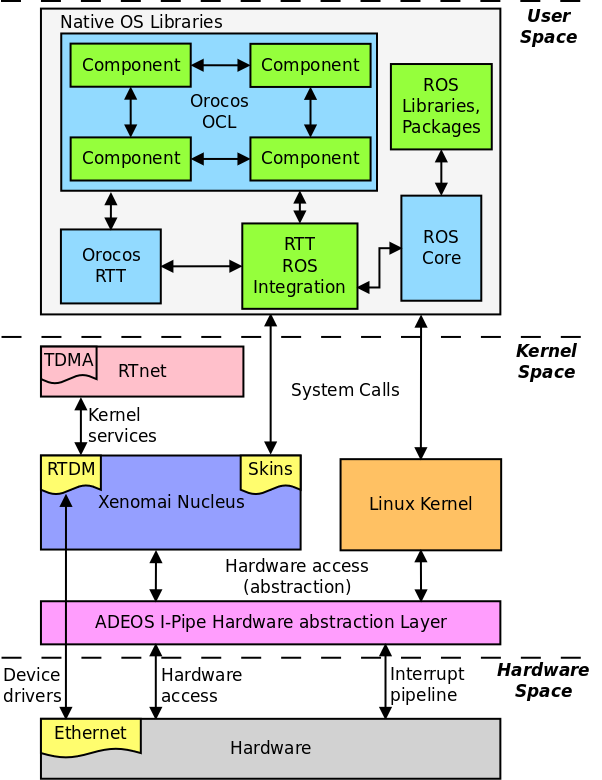
\includegraphics[width=250px,keepaspectratio]{imagens/VILMA_ENV_OVERVIEW_NET.png}
	\caption{VILMA platform infrastructure.}
	\label{fig:VILMA_ENV_OVERVIEW_NET}
\end{figure}

%
% linux
\subsection{Linux}\label{subsec:linux}

Linux is an operating system. It is the software on a computer that enables applications and the computer operator to access the devices on the computer to perform desired functions. The operating system (OS) relays instructions from an application to, for instance, the computer's processor. The processor performs the instructed task, then sends the results back to the application via the operating system \cite{linux_barabanov1997}.

%One of the most noted properties of Linux is where it can be used. Windows and OS X are predominantly found on personal computing devices such as desktop and laptop computers. Other operating systems, such as Symbian, are found on small devices such as phones and PDAs, while mainframes and supercomputers found in major academic and corporate labs use specialized operating systems such as AS/400 and the Cray OS.

Linux, which began its existence as a server OS and Has become useful as a desktop OS, can also be used on all of these devices. “From wristwatches to supercomputers”, is the popular description of Linux' capabilities. \cite{linux_foundation}

%
% xenomai
\subsection{Xenomai}\label{subsec:xenomai}

Xenomai \cite{xenomai_api} is a real-time development framework cooperating with the Linux kernel, in order to provide a pervasive, interface-agnostic, hard real-time support to user-space applications, seamlessly integrated into the GNU/Linux environment. The Xenomai drivers has the RTDM (Real-Time Driver Model) which composes the following modules: CAN Devices, Real-time IPC Devices, Serial Devices, and Testing Devices \cite{rtdm_Kiszka}.
%\cite{xenomai_x_linux}.
%
% rtnet
\subsection{RTnet}\label{subsec:rtnet}

With Ethernet, the communications are not deterministic because of the collision which can occur between several host on a network with a hub, or because of the unknown latency in the case of the switch. The deterministic communication is not allowed by the Ethernet protocol because of the possibility of collisions which can occurs and supported by the mechanism CSMA/CD (Carrier Sense Multiple Access/Collision Detection) \cite{rtnet_IEEE_so53551}.

RTnet is a protocol stack which run between the Ethernet layer and the application layer (or IP layer) with hard real-time requirements \cite{rtnet_org}. It aims, through the use of time intervals (time-slots), is to make deterministic communication, by disabling the collision detection CSMA/CD, and prevent buffering packet in the network. 


%RTnet is a software developed to run on Linux kernel with RTAI or Xenomai real-time extension. It exploits the real time kernel extension to ensure the determinism on the communication stack. In this aim, all the instructions related to this protocol makes use real time kernel functions rather than those of Linux, which bound latencies to the execution times and latencies of interruptions which provide deterministic’s communication \cite{rtnet_from_xenomai}.


%The protocol supports both real-time and non-real-time communication. Applications are able to reserve a portion of the available bandwidth to transmit real-time data, organised in streams and requires a fully-connected communication medium, such as a common bus, Ethernet, or a radio medium, where every message sent can be received directly by all other nodes. Broadcast capabilities are needed to enable automatic addition and removal of nodes and to synchronize the nodes' clocks.\cite{rtnet_1559870}. 
%At the same time the network uses the remaining bandwidth for best-effort traffic. The network is scheduled dynamically, using standard real-time scheduling algorithms normally used to schedule tasks on a CPU.
%Nodes and streams may be flexibly added and removed. The protocol can be used in any local area environment where a distributed protocol is appropriate and where Quality of Service (QoS) support and flexibility is required \cite{rtnet_Wulf03acompact}.

%
% ros
\subsection{ROS}\label{subsec:ros}
The robot software is base on the ROS (Robot Operating System) \cite{ros_components}, an meta-operating system for robots. It provides the services like hardware abstraction, low-level device control, and message-passing between processes.
ROS is composed by the operating system commands that manage the packages, and a suite of user contributed packages (organized into sets called stacks) that implement functionality such as simultaneous localization and mapping, planning, perception, simulation etc \cite{ros_gentle_introduction}. 
%\cite{ros_bmw_sticha}.

%O Robotic Operating System (ROS) \cite{ros_willowgarage} atua como um meta sistema operativo e caixa de ferramentas (toolbox). ROS fornece várias bibliotecas que são comumente usadas em problemas robóticos. Tem muitas interfaces de comunicação entre programas como o modelo publisher-subscriber, cliente-servidor, cliente-servidor assíncrono, filas de dados, relógios e gerenciador de tarefas cíclicas. Além disso, também fornece interfaces gráficas múltiplas com ferramentas para ajudar o desenvolvimento. As ferramentas podem ser usadas no tempo de execução ou armazenados para posteriores processamentos. Esta ferramenta tem licença Apache e foi a selecionada para fazer os caminhos entre os programas principalmente por sua rápida curva de aprendizagem, o suporte da comunidade livre e dos desenvolvedores, a possibilidade de usar ferramentas e módulos já desenvolvidos e a possibilidade de ser integrado com ferramentas de programação para desenvolver software com requerimentos de tempo real como o OROCOS \cite{orocos_Project_IEEE).
%
% orocos
\subsection{OROCOS}\label{subsec:orocos}
Orocos \cite{orocos_Project_IEEE} is the acronym of the Open Robot Control Software project. The project's aim is to develop a general purpose, free software, and modular framework for robot and machine control. The Orocos project supports 4 C++ libraries \cite{orocos_manual}: the Real-Time Toolkit, the Kinematics and Dynamics Library, the Bayesian Filtering Library and the Orocos Component Library.
The Orocos Real-Time Toolkit (RTT) is not an application in itself, but it provides the infrastructure and the functionalities to build robotics applications in C++.
The emphasis is on real-time, on-line interactive and component based applications. %\cite{orocos_Cobem}.

The integration between the OROCOS framework and the ROS system can be performed using \textit{rtt\_ros\_integration} \cite{rtt_ros_integration}. Briefly, ROSE is used to create a communication interface between the components and the OROCOS system performs an encapsulation of the real-time kernel API (Xenomai), enabling the definition and implementation of real-time tasks or not.

%Uma breve descrição sobre como essa integração acontece é apresentada a seguir:

%\begin{itemize}
%	\item \textbf{Data flow} Os componentes de OROCOS possuem estruturas chamadas de \textit{data ports}, meio por onde os componentes trocam dados entre si e os processos. No sistema ROS esse mecanismo é equivalente aos \textit{nodes} , que realizam a troca de informações entre os \textit{topics}. Através da biblioteca de integração, componentes OROCOS podem publicar dados para os \textit{topics} do ROS e vice versão;
%	
%	\item \textbf{Properties} Componentes OROCOS também possuem variáveis chamadas \textit{property}, ao passo que \textit{nodes} em ROS possuem os chamados \textit{parameters}. Assim, a biblioteca torna possível que os componentes OROCOS leiam os parâmetros oriundos dos \textit{server parameter} em ROS;
%	
%	\item \textbf{Deployment} O desenvolvimento dos componentes em OROCOS são executados em combinação com os \textit{nodes} em ROS através da utilização de somente um único \textit{script} de inicialização (chamado de \textit{launch});
%	
%	\item \textbf{Generation and Building} Ambos ROS e OROCOS possuem macros e \textit{scripts} disponíveis para a geração dos componentes em OROCOS e os pacotes ROS através do meta-compilador Catkin \cite{catkin_ros} \cite{catkin_gentle_intro};
%\end{itemize}

% -------------------- NEW SECTION -------------------- 
% -------------------- NEW SECTION -------------------- 
% -------------------- NEW SECTION -------------------- 
\section{Implementation}\label{sec:implementation}

The supervisory control system performs management and collecting information from other vehicle components through a common interface that must be implemented by each of the components. Thus, it should to provide other researchers of the LMA means to that they can integrate their projects to the supervisory system enabling the management of their systems in a "transparent" way. Furthermore, after the integration of supervisory, the consumption of system resources need to be as little as possible so as not to impact the functional performance of the projects.

The supervisor should also ensure the integrity of the components required to the execution of the tasks during autonomous navigation, because of it, a message will be requested periodically to each component present in the vehicle, with the the purpose of ensuring the presence of a particular component and its proper operation.

%
% module_behavior
\subsection{A General Description of Module Behavior}\label{subsec:module_behavior}

Once requested by the driver that the vehicle operates in autonomous mode, the VIS system should request to all managed components to perform their startup procedure, this may include sensors check, test the actuators, check the presence of another component in the network, etc. Then if none of the components detects failures during its startup, they must notify the supervisory system that are initialized and ready to operate in autonomous mode, so the VIS requests all components to perform the switch to the Standby state and stay waiting for new instructions.

Once in Standby, the VIS can instruct the components go to the Shutdown state in case of failures detected by any component, or to prepare for a specific mode of operation. The components can switch to the Ready state if they have done their configuration processes that ensure its activation to the operation mode specified, as instructed by the VIS. Once the process is completed, the VIS can instruct the components that begin to operate, bringing the components to the Working state. Being in the Working state , the VIS can instruct the components to return to the Standby state if the exchange of the specific mode of operation is required.

Operational errors, represented by the InternalError state can occur when a component is in any of the following states: Standby, Ready and Working. Falls exclusively to the component deciding what constitutes an operational error. When an exception occurs, the VIS can instruct the component that detected the problem both so that it performs the restart procedure or its shutdown. If rebooted, the component will return to the Standby state.

Emergencies, represented by the Exception state, can occur when a component is in any of the following states: Standby, Ready, Working or InternalError. The supervisory handles an emergency in two ways, according to the seriousness of the situation or through of the decision of operator which can instruct the component to be rebooted and return it to the Standby state after the emergency is resolved, or choose to shutdown of the system.

The structure of states and transitions shown in Figure \ref{fig:VILMA_STATE_MACHINE2} must be implemented by the VIS and for each component as an event-driven software process (event-driven). The VIS module interacts with other components based on this structure to perform supervision of the vehicle's activities. These states and transitions define the behavior of the components that are managed by the VIS. However, there is no restriction for the components to have their own states and transitions. One component can have how much states and transitions are necessary for its specific activities, the only difference is that these will not be recognized by the VIS.

%Para exemplificar, considere o componente responsável pela navegação do automóvel (Planning). O estado Working do componente Planning pode ser dividido em um sub-conjunto contendo sub-estados, por exemplo, Working-open-terrain, \textit{Working-teleoperation}, etc., estes sub-estados certamente vão possuir diferentes conjuntos de tarefas. Em particular, no sub-estado \textit{Working-teleoperation}, o componente \textit{Planning} pode não possuir tarefas específicas, ou seja, uma transição "vazia". No entanto, quando o VIS requisitar que todos os componentes realizem a transição para o estado \textit{Working} com o veículo operando em modo \textit{Teleoperation}, o componente \textit{Planning} move-se para esse estado, embora internamente esta transição possa ser indiferente quanto a transição realizada a partir do estado \textit{Standby}.

By adopting the state diagram and transitions presented in Figure \ref{fig:VILMA_STATE_MACHINE2} as a standard of behavior interface between the VIS and other components of the VILMA project, their internal activities becomes transparent to the supervisory system, ensuring the supervision of their activities without that the VIS needs to interfere in the structure and operations of each individual component.

%
%
\subsection{VIS Software Processes}\label{subsec:vis_software_processes}

The VIS module consists of two software processes, one based on the event-driven process, which has the purpose to provides the coordination of the activities between components signaling the exchange of their states. The other one is based on periodic process, periodic-tasks, for monitoring the integrity of the components present in VILMA architecture.

The event-driven process is responsible for performing four tasks:
\begin{enumerate}
	\item To manage the switch sequences of vehicle operating modes.
	\item To manage the transition between the operational states of the other components.
	\item Perform routing of data between the components.
	\item Collect informations about the vehicle status and its components.
\end{enumerate}

The periodic process is responsible for continuously monitoring the integrity of the other components at the entire time in which the vehicle is running. The verification of other components is performed through the time-stamped messages, called heartbeat, in a predefined frequency. If the period of arrival heartbeats of a component match the preset value, then the VIS module assumes that the particular component is functioning normally.

If the supervisor does not receive the heartbeat of a component, then the VIS will assume that particular component is not working properly, so the supervisor will instruct all the components to move to the Standby state, to evaluate the possible failure. The periodic process of VIS module need to send a heartbeat message to VNS module so that it can monitor the operational health of the VIS, if the VIS heartbeat messages do not arrive at VNS then it must instruct the system to the emergency procedure.

%To illustrate the applicability of the proposed supervisory control system, we consider a simple example with the scenario as shown in Figure 8. We assume that the vehicle is given a mission to reach some target through several waypoints sequentially. Upon receiving the mission to go to the target place, the mission planner depending on a satellite-based digital map will produce a task list that relates to a series ofwaypoints “w101, wl02, w103, ~104‘: which is a rough trajectory that the vehicle can traverse through, The task list and the related task specifications could be obtained accordingly, as shown in Table 1.

%Using the advanced functions “Goto” from the behavior library, the “AwlOl” task could be simply described as “Goto(SPEED, wlol)”, which means to go to the waypoint denoted by wlOl’s coordinate at a speed limited by the value indicated by “SPEED. Under the supervision of the module coordinator, the CIC will instruct all related modules to enter “Working” state and thcn call the parameterized “Goto” function. With the positioning and terrain information, the vehicle will automatically begin the “cross country” behavior and adjust to the suitable moving speed, which is the given max speed for it is traversing on plain. To save power and

%computational resource, only the necessary sensor, i.e. the UTVM’s stereovision device will he used. The CCD camera for road segment module (RSM) will be off at this moment. When the vehicle is within a given close distance to the waypoint “wlol”, the “AwlOl” task is completed. The execution of the next task is similar to the fmt one. When starting the task “AwlOY, the built-in behavior supervisor of “Goto” function will automatically switch to the “road following” behavior since a road is nearby. .Only RSM’s CCD will be used and the stereovision device will be tumed off temporarily. After completing task “AWIO~”, the vehicle will go back to “cross country” behavior for task “ A w l W . When entering the grassland terrain, the “cross country” function will automatically adjust the speed to a lower level

To illustrate this scenario, assume that the frequency of heartbeat messages to every components (excluding VIS) is set to with $1Hz$. This selection should be based on taking into consideration the distance that the vehicle will go through as soon that the failure of a component is detected by the VIS until the moment when the vehicle is fully stopped. This displacement will be called by braking distance (fail-stop).

Assume that the speed is defined by \textit{s} in \textit{km/h} and the distance of vehicle stopped by \textit{d} \textit{meters}. With a frequency of \textit{1Hz} to heartbeats messages, the VIS module will be able to detect a fault in one component for each 1 second. During the check time and under ideal conditions, the vehicle will have traveled a distance of \textit{1000s/3600} meters until its complete stop. Assuming that the needed time required for VIS instructs the system responsible for the actuators that perform the full stop of the vehicle is close to zero, then the fail-stop distance will be \textit{d + (1000s / 3600) meters}. Still as an example, assuming \textit{s = 10km/h}, \textit{d = 4m} and \textit{(1000s/3600) = 2.8m}. Thus the fail-stop distance when the vehicle is moving at speed of \textit{10km/h} will be \textit{4+2.8 = 6.8} meters in ideal conditions.
% -------------------- NEW SECTION -------------------- 
% -------------------- NEW SECTION -------------------- 
% -------------------- NEW SECTION -------------------- 
\section{Conclusion}\label{sec:conclusion}

The discussion about the supervisory control system that provides a deterministic behavior for the other autonomous vehicle systems illustrates how the robustness and security of the VILMA project can be enhanced using the methodologies presented. In this sense, the study and modeling for supervisory control system that composes the proposed architecture for VILMA vehicle development platform and its preliminary implementation in order to meet their goal was introduced, perform autonomous operations in Earth environment safely.

Through the proposed architecture, it is possible to get the management of the systems that compose the VILMA vehicle by adopting a uniform interface modeled by FSMs using generic transitions to switch states for tasks performed on every vehicle component. The state machine model represents the behavioral set that the components managed by the VIS system will implement, making the system has a high degree of determinism, i.e., the vehicle will have an expected behavior during the execution of all their tasks.

Furthermore, we showed that this architecture can ease the implementation for more sophisticated control strategies using formal techniques, as in the case of the DES, where the supervisory control based on discrete event methodology can raise the degree of autonomy of the vehicle, and represents a next step in the development of intelligent autonomous vehicle VILMA.

We also proposed a development platform composed of a technological scaffold focusing on the goal of making the work of the LMA research group standardized, consolidating the agility, the low cost for the development of the VILMA prototype and its continuity, since all the tools are well documented and widely spread. These technologies are widely used and consolidated in industrial equipments and research groups.

The integration between the low-level systems (Linux, Xenomai, Ethernet and RTnet), enables the achievement of results within the scope of the critical real-time systems with distributed processing, ensuring the requirements for the viability of the application. The integration between the user-level libraries (ROS and OROCOS), strengthens the idea of flexibility and simplification to the development of researches developed in the LMA, initially this integration is based solely on features in to the data flows between the components of this two frameworks.

%Enquanto ROS possui bom suporte para a componentes distribuídos através da rede Ethernet, OROCOS oferece suporte à tarefas de comunicação entre componentes que necessitem de garantias temporais. Isso combina o melhor dos dois mundos: o controle em tempo real de baixo nível é tratado por um conjunto de componentes OROCOS-RTT que controla diretamente a troca de estados, gerencia os modos de operação adequados, verifica constante da integridade de cada sistema e ainda torna a comunicação entre os componentes visível para toda a rede dos sistemas ROS.

%Por fim, a integração torna os componentes OROCOS como sendo componentes ROS, sem que haja quebra nos requisitos de tempo real entre os componentes OROCOS-RTT. Permitindo que sejam utilizadas as diversas ferramentas desenvolvidas para ROS, por exemplo, \textit{rviz} e \textit{rxplot}, para visualizar a comunicação entre os controladores.

% -------------------- NEW SECTION -------------------- 
% -------------------- NEW SECTION -------------------- 
% -------------------- NEW SECTION -------------------- 
% use section* for acknowledgment
\subsection*{Acknowledgment}\label{sec:acknowledgment}
The authors would like to thank...
% trigger a \newpage just before the given reference
% number - used to balance the columns on the last page
% adjust value as needed - may need to be readjusted if
% the document is modified later
%\IEEEtriggeratref{8}
% The "triggered" command can be changed if desired:
%\IEEEtriggercmd{\enlargethispage{-5in}}
% references section
% -------------------- NEW SECTION -------------------- 
% -------------------- NEW SECTION -------------------- 
% -------------------- NEW SECTION -------------------- 
\bibliographystyle{IEEEtran}
\bibliography{referencias}

% that's all folks
\end{document}